%% ------------------------------------------------------------------------- %%n
\chapter{Introdução}
\label{cap:introducao}


\section{Contexto}
\label{sec:intro_contexto}



O estudo de Plâncton é de grande importância na comunidade científica, principalmente na oceanografia. O nome plâncton vem do Grego planktos e significa errante, que vaga ou flutua. Caracteriza-se, assim, por organismos planctônicos os que não possuem o poder de locomoção suficiente para evitar o transporte passivo pelas massas de água [\cite{calazans2011organismos}].  A importância do estudo dessas criaturas se dá não somente por serem responsáveis por terem papel fundamental no ciclo de carbono com cerca de 45\% do oxigênio produzido mundialmente [\cite{brierleyplankton}],  através da fotossíntese do fitoplâncton, mas também pela grande diversidade de classes e de características como forma, tamanho e até da natureza do local de coleta [\cite{calazans2011organismos}]. 

O plâncton é taxonomicamente diverso [\cite{brierleyplankton}]. Dentre os grupos temos o fitoplâncton (plantas), o zooplâncton (animais), o bacterioplâncton (bactérias e algas cianobactérias) e o virioplâncton (vírus aquáticos). Embora possam existir tamanhos maiores, a maioria deles são muito pequenos, variando de alguns micrômetros a 5 mm de comprimento. Além disso, existem muitas maneiras de classificar esses organismos, como em função do seu tamanho ou aspectos ecológicos [\cite{calazans2011organismos}].


A amostragem de criaturas marítimas é datada desde 1829, quando Thompson utilizou uma rede para coletar larvas de crustáceos e de cracas [\cite{brierleyplankton}]. Mas foi Victor Hensen, em 1887, o primeiro pesquisador a desenvolver, de fato, um sistema para coleta de amostras de plâncton [\cite{benfield2007rapid, wiebe2003hensen, allen1919contribution}]. Naquela época estavam interessados em responder três questões fundamentais: i) quais organismos planctônicos estão presentes no mar? ii) quantos de cada tipo estão presentes? e iii) como a composição de plâncton muda com o passar do tempo?  [\cite{benfield2007rapid}]. Essas questões continuam atuais e graças ao avanço de sistemas e equipamentos de coleta, assim como de técnicas computacionais, há um grande esforço científico para responder à essas perguntas.


Ao longo dos anos, visando o estudo desses microrganismos, foram desenvolvidas diversas maneiras de se fazer a amostragem de plâncton como, através de garrafas, redes, bombas de sucção e sistemas ópticos [\cite{calazans2011organismos}]. A figura ~\ref{fig:amostragem_planctons} mostra o exemplo de uma rede planctônica. É interessante notar que nos últimos anos houve uma proliferação em sistemas ópticos. Esses sistemas permitem, por exemplo, que algumas espécies de planctôns, por serem muitos delicadas, possam ser preservadas e ter suas imagens capturadas, o que nem sempre é possível com outras técnicas [\cite{benfield2007rapid}].


\begin{figure}
  \centering
  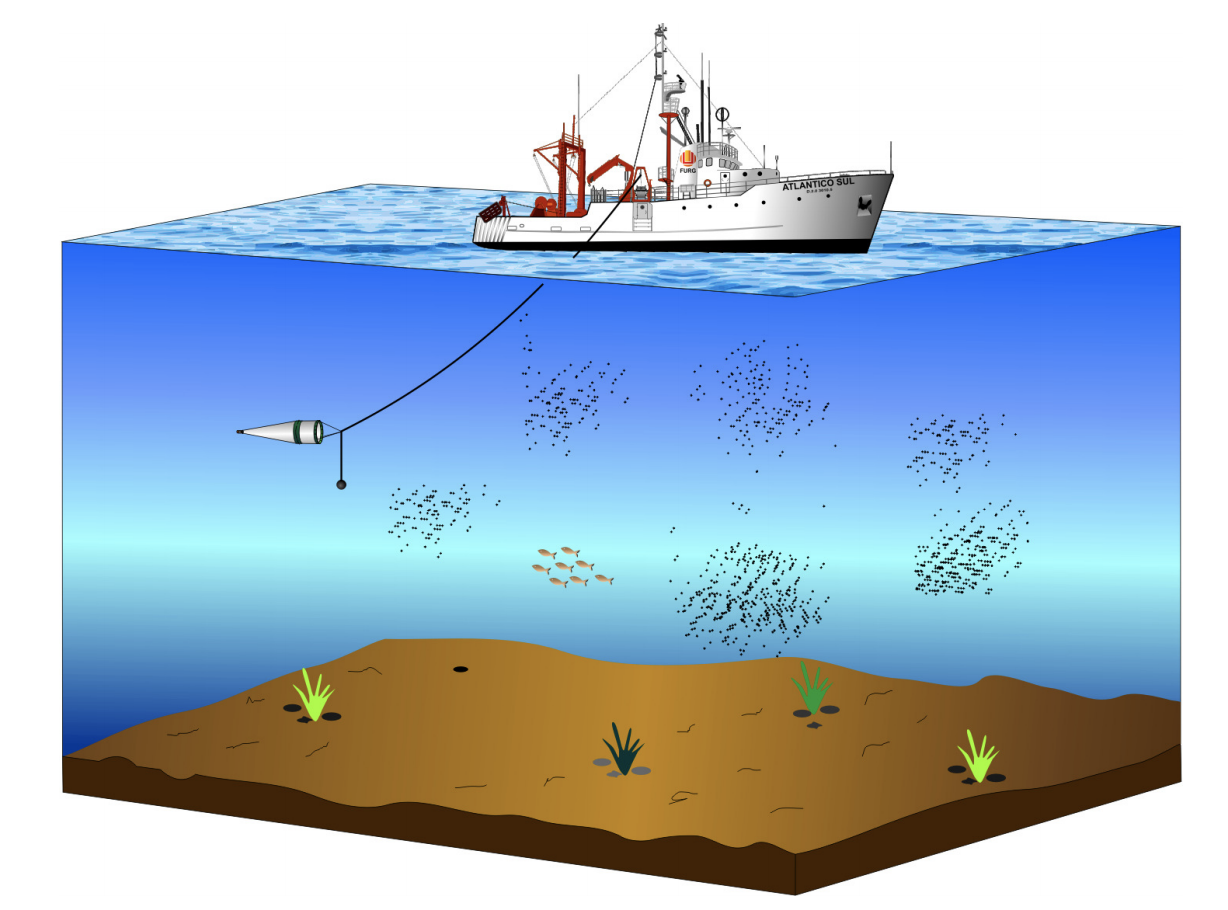
\includegraphics[width=.8\textwidth]{figures/amostragem_planctons.png}
  \caption{Rede Planctônica (Calazans, 2011)}
  \label{fig:amostragem_planctons}
\end{figure}


\section{Problema}
\label{sec:intro_problema}

Após a fase de coleta, através de sistemas ópticos, temos imagens de milhares de plâncton. Uma importante tarefa relacionada ao processamento e análise dessas imagens é a identificação, por exemplo, da espécie de plâncton, tarefa comumente conhecida como classificação. Para que isso seja feito é necessário que um profissional especialista faça a análise. Entretanto, devido à grande quantidade de imagens, essa tarefa manual se torna impraticável. Diante desse quadro, as abordagens utilizadas para classificação baseiam-se em técnicas de aprendizado de máquina. Em particular, as técnicas de aprendizado supervisionado [\cite{jeffries1980computer, jeffries1984automated, berman1990image, tang1998automatic, luo2003learning, davis2004real, grosjean2004enumeration, luo2005active, hu2005automatic, blaschko2005automatic, hu2006accurate, sosik2007automated, bell2008assessment, soh2008segmentation, al2016plankton, luo2017automated, al2018intelligent}]


As técnicas de aprendizado supervisionado geram algoritmos, também denominados classificadores, que, dada uma imagem a ser classificada, devolvem um rótulo de classe que corresponde à identificação do organismo presente na imagem. Para que seja possível gerar um classificador é necessário um conjunto de dados previamente rotulados. Esse conjunto será utilizado na fase de treinamento, que é o processo de ajustes dos parâmetros de um algoritmo. Tipicamente, rotula-se manualmente um subconjunto de um grande volume de imagens e, em seguida, utiliza-se esse subconjunto rotulado. Os classificadores podem, então, ser utilizados para classificar o restante das imagens [\cite{jeffries1980computer, jeffries1984automated, berman1990image, tang1998automatic}]. A figura XXXX mostra esse fluxo. 


O problema é que o classificador gerado a partir deste processo não é perfeito e pode ser que ele classifique imagens erroneamente. Mesmo que procure-se encontrar uma boa taxa de acerto para determinado caso, pode ser que os classificadores existentes não tenham desempenho satisfatório e precisem ser melhorados ou redesenhados. Além disso, as características das imagens de plâncton podem variar, dependendo do local ou da época, ou ainda, do tipo de equipamento utilizado na coleta. Quando essas situações ocorrem é necessário uma nova rotulação das imagens, o que requer muito esforço de um profissional especialista e pode levar muito tempo. Nesse sentido, muita pesquisa tem sido feita com relação a esse problema onde temos uma grande quantidade de dados coletadas, mas com pouquíssimos ou nenhum deles com rótulos. 



\section{Proposta}
\label{sec:intro_proposta}


As técnicas na área de aprendizado de máquina conhecidas na literatura para se trabalhar com uma quantidade nula ou limitada de dados rotulados a fim de criar um classificador concentram-se no Aprendizado Ativo e no Semi-supervisionado. Dentro desse escopo, uma das vantagens do Aprendizado Ativo é que ele pode incluir um humano especialista como o papel do oráculo. Isso é extremamente importante em problemas desse tipo [\cite{saito2014active}], como de classificação de plâncton. Além disso, estudos mostram que a inclusão de conhecimento humano especializado pode aumentar a acurácia dos modelos [\cite{benfield2007rapid}].

Trabalhos recentes tem como objetivo incluir um papel mais ativo do humano no framework do aprendizado ativo. Essa não é uma questão nova [\cite{castro2009human, dasgupta2011two}] e estudos demonstram resultados positivos na intersecção do aprendizado ativo com a ciência cognitiva [\cite{kottke2018other}]. Uma maneira interessante de se fazer isso é através da interação do humano com a visualização de dados [\cite{yang2018visually, bernard2018comparing, weigl2016mapview}].  


A proposta desta dissertação é desenvolver um método efetivo para rotulação e classificação de imagens de plâncton, usando técnicas de aprendizado ativo, aprendizado semi-supervisionado e interação ativa de usuários. Para isso, a ideia central consiste em encontrarmos boas representações das imagens que capturem similaridade entre os organismos, formas interessantes de visualizar as estruturas e padrões presentes no conjunto de dados (através de projeções 2D ou galeria de imagens), juntamente com mecanismos de interação nos quais o usuário especialista poderá informar os rótulos. As imagens rotuladas podem, assim, ser utilizadas no framework de aprendizado ativo para a produção de um classificador e esse processo, que consiste na propagação de rótulos, teria como objetivo agilizar a rotulação das imagens restantes. O objetivo principal é diminuir a interação do usuário quando comparado com o framework padrão de aprendizado supervisionado. 

Para validar o método, o aprendizado ativo padrão, no qual o usuário interage apenas como oráculo, será utilizado como baseline. Também compararemos com a seleção feita de forma randômica, que é uma forma de validação normalmente utilizada. No método a ser desenvolvido espera-se uma interação mais ativa do usuário, na qual a escolha sobre quais amostras rotular fica restrita ao usuário, e, portanto, conjectura-se que um número menor de interações seja suficiente para se obter classificares com desempenho similar ao obtido com a classificação do framework padrão.

%\section{Trabalhos Relacionados}
%\label{sec:intro_relacionados}

%To do: citar trabalhos relacionados, principalmente nos últimos anos. Falar, por exemplo, do trabalho da Priscila. 


\section{Organização}
\label{sec:intro_organizacao}

Esta qualificação está definida da seguinte maneira: o capítulo dois faz uma revisão teórica do Aprendizado Ativo e comenta a respeito das principais limitações e desafios. O capítulo 3 aborda a descrição do problema e a proposta. O capítulo 4 mostra alguns experimentos e resultados preliminares, enquanto o último capítulo fala do plano de trabalho e cronograma.